\documentclass[fontsize=12bp, paper=a4]{scrarticle}
\usepackage[utf8]{inputenc}

\usepackage[english,main=serbian]{babel}
\usepackage[left=2cm, right=2cm, top=3cm, bottom=3cm]{geometry}
\usepackage[automark]{scrlayer-scrpage}
\usepackage{ragged2e}
\usepackage{amsmath}
\usepackage{mathabx}
\usepackage{hyperref}
\usepackage{graphicx}
\usepackage{wrapfig}
\usepackage{amssymb}
\usepackage{listings}
\usepackage{xcolor}
\usepackage{csquotes}
%\usepackage[backend=biber, style=numeric]{biblatex}

%
\definecolor{codegreen}{rgb}{0,0.6,0}
\definecolor{codegray}{rgb}{0.5,0.5,0.5}
\definecolor{codepurple}{rgb}{0.58,0,0.82}
\definecolor{backcolour}{rgb}{0.95,0.95,0.92}

\lstdefinestyle{mystyle}{
    backgroundcolor=\color{backcolour},   
    commentstyle=\color{codegreen},
    keywordstyle=\color{magenta},
    numberstyle=\tiny\color{codegray},
    stringstyle=\color{codepurple},
    basicstyle=\ttfamily\footnotesize,
    breakatwhitespace=false,         
    breaklines=true,                 
    captionpos=b,                    
    keepspaces=true,                 
    numbers=left,                    
    numbersep=5pt,                  
    showspaces=false,                
    showstringspaces=false,
    showtabs=false,                  
    tabsize=2
}

\lstset{style=mystyle}

\renewcommand\lstlistingname{Implementacija}
\renewcommand\lstlistlistingname{Implementacija}

%

\graphicspath{ {./images/} }

%
\title{Seminarski rad} 
\subtitle{iz predmeta Teorijske osnove veštačke inteligencije}

\begin{document}

\begin{titlepage}
    \vspace{\stretch{1}}
    
    \begin{center}
        
        \vspace*{8cm}
        
        \large{Univerzitet u Kragujevcu}
        
        \vspace*{1cm}

        {\bfseries \LARGE Domaći zadatak}
        
        \large{iz predmeta Sistem za podršku odlučivanju}
        
        \vspace*{1cm}
        \large{Tema:}

        \Large{Implementacija klasifikacionih algoritmima sa nadgledanim učenjem}


        \vspace*{2cm}
    \end{center}
    \hfill{\parbox[s]{8cm}{

    mentori: 
    \begin{tabular}{l}
        \\
        \\
        Ognjen Pavić, \\
        prof. dr. Tijana Geroski, \\
        prof. dr. Nenad Filipović 
    \end{tabular}
    
    student: \begin{tabular}{l}
        Željko Simić 3vi/2023
    \end{tabular}
    }}

    \hspace*{\fill} 

    \vspace*{2cm}

    \begin{center}
        Kragujevac 2024.
    \end{center}
\end{titlepage}


\setcounter{page}{1}
\justifying
\linespread{0.9}
\cfoot[\pagemark]{\pagemark}
\ofoot[]{}
\ohead[]{Željko Simić 3vi/2023}
\chead[]{}
\ihead[]{Univerzitet u Kragujevcu}
%
\justifying

\section{Uvod}

Dat je \verb|``Social_Network_Ads.csv''| dataset.\cite{dataset} Namenjen za sagledanje  U sebi sadr\i 400 instanci (uzoraka), a ima u sebi za svaki po 4 kolona atributa (posmatran kao ulazna vrednost):
\begin{itemize}
    \item \verb|User ID| - Ukazuje na udeljeni jedinstveni identifikator korisnika posmatranog sistema. \textbf{Biće izbačen pri sagledanju i neće biti uzet u obzir};
    \item \verb|Gender| - Ukazuje na pol korisnika, kategoričkih vrednosti (\verb|Male, Female|);
    \item \verb|Age| - Ukazuje na starost korisnika, sa kontinualnim vrednostima u domenu $[18,60]$
    \item \verb|EstimatedSalary| - Ukazuje na starost korisnika sistema, kontinualna vrednost u domenu od $[15000, 150000]$
\end{itemize}
i 1 ciljnu vrednost (posmatran kao izlaznu vrednost):
\begin{itemize}
    \item \verb|Purchased| - Ukazuje da li je korisnik sistema pazario proizvod za kog važi ovaj skup podataka, koji je kategorička vrednost \verb|0, 1| - što dovodi klasifikacije koje se obavljaju budu \textbf{binarne}. 
\end{itemize}

\newpage
\section{Metodologija}


% korelacija ulaza naspram izlaza

% distribucija po starosti koji nisu / jesu kupili 
% distribucija po plaćenosti koji nisu / jesu kupili 


Uz tekst seminarskog rada je priložen izvorni kod (na putanji \verb|./src/main.py|) koji će se ovde sagledati. Implementacija 1. u sebi sadrži deklaracije uvedenih modula iz kojih će biti pozivane njihove komponente u daljem radu (praktično realizovanje teorijskog rada na ovu temu\cite{mojRad}). Korišćen je objektni tip podataka \verb|pandas.DataFrame|\cite{pandasDF} kojim će biti urađeno strukturno skladištenje (sa metodom \verb|pd.read_csv(putanja_csv_fajla_skupa_podataka)|) i manipulisano elementima skupa podataka koji je bio pomenut u uvodu. Biće izvršeno predprocesiranje u kom spada eliminisanje \verb|User ID| atributa, enkodiranje \verb|Gender| atributa (da bi bio prikladan za dalji rad sa klasifikatorima iz vrednosti tipa string-a u broj)\cite{labelEncoding}, podela skupa podataka uz \verb|train_test_split(...)| na trening i test skupove podataka po nekoj razmeri $8:2$ za ulazne i izlazne vrednosti klasifikacija.\cite{train_test_split}


\begin{lstlisting}[language=Python, caption=Predprocesiranje podataka i navođenje modula koji će se koristiti]

import pandas as pd
from sklearn.linear_model import LogisticRegression
from sklearn.tree import DecisionTreeClassifier
from sklearn.ensemble import RandomForestClassifier
from sklearn.naive_bayes import GaussianNB
from sklearn.naive_bayes import MultinomialNB
from sklearn.naive_bayes import BernoulliNB
from sklearn.naive_bayes import CategoricalNB
from sklearn.naive_bayes import ComplementNB
from sklearn.svm import SVC
from sklearn.neighbors import KNeighborsClassifier
# from sklearn.neighbors import RadiusNeighborsClassifier

from sklearn.model_selection import train_test_split
import seaborn as sb
import matplotlib.pyplot as plt
import numpy as np
from sklearn.metrics import classification_report
from sklearn.metrics import confusion_matrix
from sklearn.preprocessing import LabelEncoder
from sklearn.model_selection import GridSearchCV

...

dataframe = pd.read_csv('./Social_Network_Ads.csv')
# storing all dataframe without user ids
data = dataframe.iloc[:,1:]

le = LabelEncoder()
le.fit(data.iloc[:, 0])

# Encoding to numerical binary values for the purposes of dealing with NaiveBayes classificators 
# https://scikit-learn.org/stable/modules/generated/sklearn.preprocessing.LabelEncoder.html

encoded_genders = le.transform(data.iloc[:, 0])
data[data.columns[0]] = encoded_genders

...

x_train, x_test, y_train, y_test = train_test_split(
		data[data.columns[:-1]],
		data[data.columns[-1]],
		test_size=0.2
)
\end{lstlisting}

% \begin{lstlisting}[language=Python, caption=Predprocesiranje podataka i navođenje modula koji će se koristiti]
% \end{lstlisting}

\vbox{}

\vbox{}

U implementaciji 2. vrši se generisanje slika 1. (za korelaciju među features-ima po verovatonosnoj distributivnoj funkciji (PDF) na target vrednost \verb|Purchased|), 2. (za distribuciju naspram feature-a \verb|Age| i target vrednosti), 3. (za distribuciju naspram feature-a \verb|EstimatedSalary|). Ovo sve je obavljeno uz metode \verb|seaborn.pairplot| za sliku 1.\cite{pairplot} i \verb|seaborn.displot| za slike 2. i 3.\cite{displot}

\begin{lstlisting}[language=Python, caption=Navođenje načina vizuelizacija za sliku \texttt{1., 2. i 3.}]
    # visualization of correlation
    sb.pairplot(data, hue="Purchased")

    # visualization of distribution against Age feature and target value
    sb.displot(data, 
    hue = "Purchased", 
    palette = "Spectral",
    x = data['Age'],
    kind = 'kde',
    fill = True)
# visualization of distribution against EstimatedSalary feature and target value
sb.displot(data, 
hue = "Purchased", 
palette = "Spectral",
			x = data['EstimatedSalary'],
			kind = 'kde',
			fill = True)
\end{lstlisting}

Na slici 1. je moguće uočiti da PDF za feature \verb*|Gender| vrednosti među sobom (\verb|0| za \verb|Male|, a \verb*|1| za \verb*|Female|) po \verb*|Purchased| vrednosti ukazuje na malo veću kupovnu moć posmatranog proizvoda kod muškaraca, nego kod žena.

Za PDF \verb*|Gender| naspram \verb*|Age| po \verb|Purchased| može se videti da kupovna moć ovog proizvoda je kod muškaraca i kod žena u domenu od 45+ godina, ali kod muškaraca možda malo prostranjenije po godinama.

Za PDF \verb*|Gender| naspram \verb*|EstimatedSalary| po \verb|Purchased| može se videti da kupovna moć ovog proizvoda je kod muškaraca i kod žena u domenu od 75000+, ali da ne kupuju oba pola u domenu od [50000, 75000].

Za PDF \verb*|Age| među sobom po \verb|Purchased| može se videti da kupovna moć ovog proizvoda je najveća negde oko 50 godina, ali i da ne kupuju najviše sa 30 godina što je i dominantnije. Što je i prikazano na slici 2.

Za PDF \verb*|Age| naspram \verb*|EstimatedSalary| po \verb|Purchased| može se videti da kupovna moć ovog proizvoda je kod starosti [40, 60] svih raspoloživih prihoda, ali da ne kupuju domenu prihod od [0, 75000] kod onih koji su u starosti od [20, 40] godina.

Za PDF \verb*|EstimatedSalary| među sobom po \verb|Purchased| može se videti da kupovna moć ovog proizvoda je najveća među prihodima od 100000, ali i da ne kupuju najviše sa prihodom 75000 što je i dominantnije. Što je i prikazano na slici 3.

\begin{figure}[h!]
    \centering
    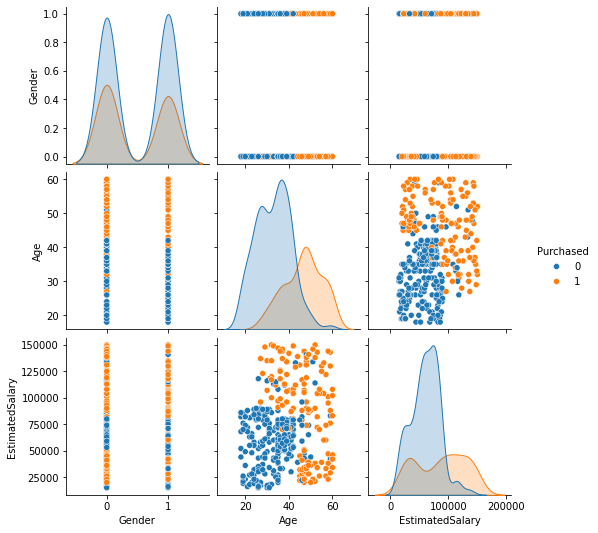
\includegraphics[width=0.75\textwidth]{32.png}
    \caption{\centering Vizuelizacija za korelaciju među features-ima po verovatonosnoj distributivnoj funkciji (PDF) na target vrednost \texttt{Purchased}}
\end{figure}      

\begin{figure}[tbp!]
    \centering
    \begin{minipage}[b]{0.45\textwidth}
        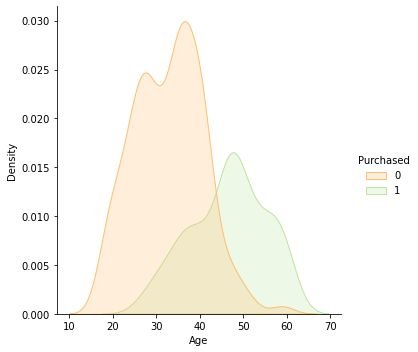
\includegraphics[width=1\textwidth]{30.png}
        \caption{\centering Vizuelizacija za distribuciju naspram feature-a \texttt{Age} i target vrednosti}
    \end{minipage}
    \hfill
    \begin{minipage}[b]{0.45\textwidth}
        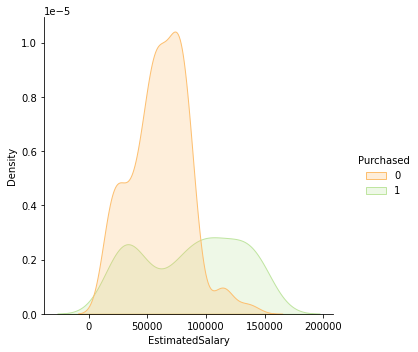
\includegraphics[width=1\textwidth]{31.png}
        \caption{\centering Vizuelizacija za distribuciju naspram feature-a \texttt{EstimatedSalary} i target vrednosti}
    \end{minipage}
\end{figure}   
\newpage
U implementaciji 3. je realizovana klasifikacija \textbf{logističkom regresijom sa optimizacijom hiperparametara} korišćenjem \verb|LogisticRegression|\cite{LR} i \verb|GridSearchCV|\cite{GCV}. U promenljivu \verb|param_grid| smešteni su parovi ključ, vrednost za koncepte:
\begin{itemize}
    \item \verb*|C| - podešena jačina inverzne regulacije, pozitivna decimalna vrednost. Manja vrednost jača regulacija. \verb|np.logspace(...)| daje listu elemenata $10^{-1}, ..., 10^{-9}$ gde je stepen 10, ali izvodilac je određen $ln(\verb|broj_elemenata|) \over ln(\verb|stepen|)$ korakom.\cite{npLogspace}
    \item \verb*|penalty| - podešeni su određeni režimi penala (kazne), l2 bi inače bio podrazumevan, ovi penali mogu da ne rade za određene rešavače.
    \item \verb|solver| - podešeni rešavači, tj. algoritmi za optimizacioni problem, gde je \verb*|lbfgs| podrazumevan.
    \item \verb*|class_weight| - podešena pristrasnost za neku ciljanu vrednost \verb*|Purchased|-a, npr. u ovom slučaju samo za vrednost \verb*|0|, tj. nekupljenog proizvoda je manja pristrasnost - od $20\%$, nego kod vrednosti \verb|1|, tj. kupljenog - od $80\%$.
    \item \verb|l1_ration| - koristan samo u slučaju režima penala \verb|elasticnet| u kom je korišćen kao miksing parametar kao što je u teorijskom domaćem zadatku pričano o \textit{regularizacije elastične mreže $\rho$}. 
    \item \verb*|multi_class| - moguće podrazumevano automatski, ali podešava ishode po binarnom ili po višeklasnom funkciji PDF. Priča vezana oko binarne, OVR, multinomijalne logističke regresije u teoriji. 
\end{itemize} 
\verb*|GridSearchCV| radi isprobavanje svakog ponaosob hiperparametra nad klasifikatorom i stratifikovan cross-validation postupak na 10 fold-ova. Izvlači se najbolji ishod evaluacija pri predviđanju test skupom nad obučenim modelom. Kasnije će biti diskutovano o analizi koja je obrađena uz \verb|classification_report(...)| i \verb|confusionMatrix(...)| - koji je korisnički definisana funkcija prikazana u implementaciji 4. gde se vrši iscrtavanje konfuzione matrice (pogotka ciljanih vrednosti naspram predviđenih modelom i stvarnih vrednosti iz trening skupa).
\begin{lstlisting}[language=Python, caption=Logistička regresija sa optimizacijom hiperparametara.]
    print('Logistic Regression prediction:')
LR = LogisticRegression()
param_grid = {
    'C': np.logspace(-1, -9, num=10),
 	'penalty': ['l1', 'l2', 'elasticnet'],
 	'solver': ['lbfgs', 'liblinear', 'newton-cg', 'newton-cholesky', 'saga'],
 	'class_weight' : ['balanced', 'None', {0: 0.2, 1:0.8}],
 	'l1_ratio': [0, 0.1, 1],
 	'multi_class': ['auto', 'ovr', 'multinomial']
 	
}
LR_grid = GridSearchCV(estimator = LR,
                       param_grid=param_grid, verbose=0,
                       cv=10, n_jobs=-1)
LR_grid.fit(x_train,y_train)
prediction=LR_grid.predict(x_test)
print('Best case:')
print(LR_grid.best_estimator_)
print()
report = classification_report(list(y_test), prediction)
print(report)

cm=confusionMatrix(list(y_test),prediction, "Logistic regression w/ optimization")
\end{lstlisting}

\begin{lstlisting}[language=Python, caption=Funkcija za generisanje konfuzione matrice.]
    
def confusionMatrix(y_true,y_pred,title):
	cm=confusion_matrix(y_pred,y_true)
	plt.figure()
	sb.heatmap(cm, annot=True, fmt='0')
	plt.title(title)
	plt.xlabel('True Value')
	plt.ylabel('Predicted Value')
    
\end{lstlisting}

U implementaciji broj 5. vrši se obična \textbf{logistička regresija} bez ikakvih optimizacija hiperparametara.
\begin{lstlisting}[language=Python, caption=Logistička regresija bez ikakvih optimizacija hiperparametara.]
    print(f'Logistic Regression prediction without optimization:')
    LR.fit(x_train,y_train)
    prediction=LR.predict(x_test)
    
    print()
    report = classification_report(list(y_test), prediction)
    print(report)
\end{lstlisting}

U implementaciji 6. je realizovana klasifikacija \textbf{stabla odlučivanja sa optimizacijom hiperparametara} korišćenjem \verb|DecisionTreeClassifier|\cite{DT} i \verb|GridSearchCV|. U promenljivu \verb|param_grid| smešteni su parovi ključ, vrednost za koncepte:
\begin{itemize}
    \item \verb|criterion| - mera za podešavanje funkcije određivanja kvaliteta podele.
    \item \verb|max_depth| - najveća dubina stabla odluke koja je uzeta u razmatranje.
    \item \verb|min_samples_leaf| - minimalan broj uzoraka u čvorovima listova u stablu, tačka podele ma koje dubine će biti uvažena ako se ustanovi toliki broj uzoraka trening skupa i sa leve i sa desne grane. Utiče na \textit{smooth}-ovanje. Zaokruživanje broja vrši na više.
    \item \verb|ccp_alpha| - parametar za primenu pri \textit{odecanju minimalne cene kompleksnoti}.
\end{itemize} 
\verb*|GridSearchCV| radi isprobavanje svakog ponaosob hiperparametra nad klasifikatorom i stratifikovan cross-validation postupak na 10 fold-ova. Izvlači se najbolji ishod evaluacija pri predviđanju test skupom nad obučenim modelom. Kasnije će biti diskutovano o analizi koja je obrađena uz \verb|classification_report(...)| i \verb|confusionMatrix(...)|.
\begin{lstlisting}[language=Python, caption=Stablo odlučivanja sa optimizacijama hiperparametara.]
DT = DecisionTreeClassifier()
param_grid = {
    'criterion': ['gini', 'entropy'],
    'max_depth': np.arange(3, 15, step=6),
    'min_samples_leaf': np.arange(1, 10, step=3),
    'ccp_alpha': [0, 0.1, 0.2]  
}
DT_grid = GridSearchCV(estimator = DT,
                       param_grid=param_grid, verbose=0,
                       cv=10, n_jobs=-1)
DT_grid.fit(x_train,y_train)
prediction=DT_grid.predict(x_test)
print('Best case:')
print(DT_grid.best_estimator_)
print()
report = classification_report(list(y_test), prediction)
print(report)

cm=confusionMatrix(list(y_test),prediction, "Decision Tree w/ optimization")

\end{lstlisting}

U implementaciji broj 7. vrši se obična \textbf{klasifikacija stabla odlučivanja} bez ikakvih optimizacija hiperparametara.
\begin{lstlisting}[language=Python, caption=Stablo odlučivanja bez ikakvih optimizacija hiperparametara.]
    print(f'Decision Tree prediction without optimization:')
    DT.fit(x_train,y_train)
    prediction=DT.predict(x_test)
    
    print()
    report = classification_report(list(y_test), prediction)
    print(report)
\end{lstlisting}
U implementaciji 8. je realizovana klasifikacija \textbf{slučajnih šuma sa optimizacijom hiperparametara} korišćenjem \verb|RandomForestClassifier|\cite{RFC} i \verb|GridSearchCV|. U promenljivu \verb|param_grid| smešteni su parovi ključ, vrednost za koncepte:
\begin{itemize}
    \item \verb|n_estimators| - broj stabala odlučivanja u šumi, podrazumeva se da bude 100.
    \item \verb|max_depth| - najveća dubina stabla odluke koja je uzeta u razmatranje.
    \item \verb|min_samples_leaf| -  minimalan broj uzoraka u čvorovima listova u stablu, tačka podele ma koje dubine će biti uvažena ako se ustanovi toliki broj uzoraka trening skupa i sa leve i sa desne grane. Utiče na \textit{smooth}-ovanje. Zaokruživanje broja vrši na više.
    \item \verb|min_samples_split| - minimalan potreban broj uzoraka da bi se desila podela, ako nije \verb*|int| tipa onda če da vrši zaokruživanje broja naviše.
    \item \verb|bootstrap| - koriste se se bootstrap uzorci pri gradnji stabala, inače je korišćen čitav skup podataka za izgradnju stabala (što je podrazumevan slučaj1).
\end{itemize} 
\verb*|GridSearchCV| radi isprobavanje svakog ponaosob hiperparametra nad klasifikatorom i stratifikovan cross-validation postupak na 10 fold-ova. Izvlači se najbolji ishod evaluacija pri predviđanju test skupom nad obučenim modelom. Kasnije će biti diskutovano o analizi koja je obrađena uz \verb|classification_report(...)| i \verb|confusionMatrix(...)|.
\begin{lstlisting}[language=Python, caption=Slučajna šuma sa optimizacijama hiperparametara.]
print('Random Forest prediction:')
RF = RandomForestClassifier()
param_grid = {
    'n_estimators': np.arange(start=4, stop=20, step=4),
    'max_depth': list(range(10, 110, 50)) + [None],
    'min_samples_split': [2, 5, 10],
    'min_samples_leaf': [1, 2, 4],
    'bootstrap': [True, False]
}
RF_grid = GridSearchCV(estimator = RF,
                       param_grid=param_grid, verbose=0, 											
                       cv=10, n_jobs=-1)
RF_grid.fit(x_train,y_train)
prediction=RF_grid.predict(x_test)
print('Best case:')
print(RF_grid.best_estimator_)
print()
report = classification_report(list(y_test), prediction)
print(report)

cm=confusionMatrix(list(y_test),prediction, "Random Forst w/ optimization")
\end{lstlisting}
U implementaciji broj 9. vrši se obična \textbf{klasifikacija slučajnih šuma} bez ikakvih optimizacija hiperparametara.

\begin{lstlisting}[language=Python, caption=Slučajne šume bez ikakvih optimizacija hiperparametara.]
print(f'Random Forest prediction without optimization:')
RF.fit(x_train,y_train)
prediction=RF.predict(x_test)
report = classification_report(list(y_test), prediction)
print(report)
\end{lstlisting}

%%%%%%%%%%%%%%%%%%%%%%%%%%%%%%%%
U implementaciji 10. je realizovana klasifikacija \textbf{Gausov naivni Bajes sa optimizacijom hiperparametara} korišćenjem \verb|GaussianNB|\cite{GNB} i \verb|GridSearchCV|. U promenljivu \verb|param_grid| smešteni su parovi ključ, vrednost za koncepte:
\begin{itemize}
    \item \verb|var_smoothing| - podešava količinu najveće disperzije svih features-a koji doprinose stabilnosti sračunavanja.
\end{itemize} 
\verb*|GridSearchCV| radi isprobavanje svakog ponaosob hiperparametra nad klasifikatorom i stratifikovan cross-validation postupak na 10 fold-ova. Izvlači se najbolji ishod evaluacija pri predviđanju test skupom nad obučenim modelom. Kasnije će biti diskutovano o analizi koja je obrađena uz \verb|classification_report(...)| i \verb|confusionMatrix(...)|.
\begin{lstlisting}[language=Python, caption=Gausov naivni Bajes sa optimizacijama hiperparametara.]
print('Gaussian Naive Bayes prediction:')

GNB=GaussianNB()
param_grid = {
    'var_smoothing': np.logspace(1, -9, num=10)
}
GNB_grid = GridSearchCV(estimator = GNB,
						param_grid=param_grid, verbose=0, 											
                        cv=10, n_jobs=-1)
GNB_grid.fit(x_train,y_train)
prediction=GNB_grid.predict(x_test)
print('Best case:')
print(GNB_grid.best_estimator_)
print()
report = classification_report(list(y_test), prediction)
print(report)

cm=confusionMatrix(list(y_test),prediction, "Gaussian Naive Bayes w/ optimization")
\end{lstlisting}
U implementaciji broj 11. vrši se obična \textbf{klasifikacija Gausov naivni Bajes } bez ikakvih optimizacija hiperparametara.

\begin{lstlisting}[language=Python, caption=Gausov naivni Bajes bez ikakvih optimizacija hiperparametara.]
print(f'Gaussian Naive Bayes prediction without optimization:')
GNB.fit(x_train,y_train)
prediction=GNB.predict(x_test)
report = classification_report(list(y_test), prediction)
print(report)
\end{lstlisting}
U implementaciji 12. je realizovana klasifikacija \textbf{multinomijani naivni Bajes sa optimizacijom hiperparametara} korišćenjem \verb|MultinomialNB|\cite{MNB} i \verb|GridSearchCV|. U promenljivu \verb|param_grid| smešteni su parovi ključ, vrednost za koncepte:
\begin{itemize}
    \item \verb|alpha| - aditivni (Laplace/Lidstone) smoothing parametar.
\end{itemize} 
\verb*|GridSearchCV| radi isprobavanje svakog ponaosob hiperparametra nad klasifikatorom i stratifikovan cross-validation postupak na 10 fold-ova. Izvlači se najbolji ishod evaluacija pri predviđanju test skupom nad obučenim modelom. Kasnije će biti diskutovano o analizi koja je obrađena uz \verb|classification_report(...)| i \verb|confusionMatrix(...)|.
\begin{lstlisting}[language=Python, caption=Multinomialni naivni Bajes sa optimizacijama hiperparametara.]
print(f'Multinomial Naive Bayes prediction:')
MNB=MultinomialNB()
param_grid = {
    'alpha': np.logspace(-1, -9, num=10)
}
MNB_grid = GridSearchCV(estimator = MNB,
						param_grid=param_grid, verbose=0, 									 		
                        cv=10, n_jobs=-1)
MNB_grid.fit(x_train,y_train)
prediction=MNB_grid.predict(x_test)
print('Best case:')
print(MNB_grid.best_estimator_)
print()
report = classification_report(list(y_test), prediction)
print(report)
\end{lstlisting}
U implementaciji broj 13. vrši se obična \textbf{klasifikacija multinomijalni naivni Bajes } bez ikakvih optimizacija hiperparametara.

\begin{lstlisting}[language=Python, caption=Multinomijalni naivni Bajes bez ikakvih optimizacija hiperparametara.]
MNB.fit(x_train,y_train)
prediction=MNB.predict(x_test)
print(f'Multinomial Naive Bayes prediction without optimization:')
report = classification_report(list(y_test), prediction)
print(report)
\end{lstlisting}
U implementaciji 14. je realizovana klasifikacija \textbf{Bernuli naivni Bajes sa optimizacijom hiperparametara} korišćenjem \verb|BernoulliNB|\cite{BNB} i \verb|GridSearchCV|. U promenljivu \verb|param_grid| smešteni su parovi ključ, vrednost za koncepte:
\begin{itemize}
    \item \verb|alpha| - aditivni (Laplace/Lidstone) smoothing parametar.
\end{itemize} 
\verb*|GridSearchCV| radi isprobavanje svakog ponaosob hiperparametra nad klasifikatorom i stratifikovan cross-validation postupak na 10 fold-ova. Izvlači se najbolji ishod evaluacija pri predviđanju test skupom nad obučenim modelom. Kasnije će biti diskutovano o analizi koja je obrađena uz \verb|classification_report(...)| i \verb|confusionMatrix(...)|.
\begin{lstlisting}[language=Python, caption=Bernulijev naivni Bajes sa optimizacijama hiperparametara.]
print(f'Bernoulli Naive Bayes prediction:')
BNB=BernoulliNB()
param_grid = {
    'alpha': np.logspace(-1, -9, num=10)
}
BNB_grid = GridSearchCV(estimator = BNB,
						param_grid=param_grid, verbose=0, 											
                        cv=10, n_jobs=-1)
BNB_grid.fit(x_train,y_train)
prediction=BNB_grid.predict(x_test)
print('Best case:')
print(BNB_grid.best_estimator_)
print()
report = classification_report(list(y_test), prediction)
print(report)
\end{lstlisting}
U implementaciji broj 15. vrši se obična \textbf{klasifikacija Bernulijev naivni Bajes } bez ikakvih optimizacija hiperparametara.

\begin{lstlisting}[language=Python, caption=Bernulijev naivni Bajes bez ikakvih optimizacija hiperparametara.]
print(f'Bernoulli Naive Bayes prediction without optimization:')
BNB=BernoulliNB()
BNB.fit(x_train,y_train)
prediction=BNB.predict(x_test)

print()
report = classification_report(list(y_test), prediction)
print(report)
\end{lstlisting}
U implementaciji 16. je realizovana klasifikacija \textbf{kategorički naivni Bajes sa optimizacijom hiperparametara} korišćenjem \verb|CategoricalNB|\cite{CatNB} i \verb|GridSearchCV|. U promenljivu \verb|param_grid| smešteni su parovi ključ, vrednost za koncepte:
\begin{itemize}
    \item \verb|alpha| - aditivni (Laplace/Lidstone) smoothing parametar.
\end{itemize} 
\verb*|GridSearchCV| radi isprobavanje svakog ponaosob hiperparametra nad klasifikatorom i stratifikovan cross-validation postupak na 10 fold-ova. Izvlači se najbolji ishod evaluacija pri predviđanju test skupom nad obučenim modelom. Kasnije će biti diskutovano o analizi koja je obrađena uz \verb|classification_report(...)| i \verb|confusionMatrix(...)|.
\begin{lstlisting}[language=Python, caption=Kategorički naivni Bajes sa optimizacijama hiperparametara.]
print(f'Categorical Naive Bayes prediction:')

CatNB=CategoricalNB()
param_grid = {
    'alpha': np.logspace(-1, -9, num=10)
}
CatNB_grid = GridSearchCV(estimator = CatNB,
						param_grid=param_grid, verbose=0, 									
                        cv=10, n_jobs=-1)
CatNB_grid.fit(x_train,y_train)
prediction=CatNB_grid.predict(x_test)
print('Best case:')
print(CatNB_grid.best_estimator_)
print()
report = classification_report(list(y_test), prediction)
print(report)


CatNB.fit(x_train,y_train)
prediction=CatNB.predict(x_test)
\end{lstlisting}
U implementaciji broj 17. vrši se obična \textbf{klasifikacija kategorički naivni Bajes } bez ikakvih optimizacija hiperparametara.

\begin{lstlisting}[language=Python, caption=Kategorički naivni Bajes bez ikakvih optimizacija hiperparametara.]

print(f'Categorical Naive Bayes prediction without optimization:')
CatNB.fit(x_train,y_train)
prediction=CatNB.predict(x_test)

print()
report = classification_report(list(y_test), prediction)
print(report)
\end{lstlisting}
U implementaciji 18. je realizovana klasifikacija \textbf{multinomijani naivni Bajes sa optimizacijom hiperparametara} korišćenjem \verb|ComplementNB|\cite{CNB} i \verb|GridSearchCV|. U promenljivu \verb|param_grid| smešteni su parovi ključ, vrednost za koncepte:
\begin{itemize}
    \item \verb|alpha| - aditivni (Laplace/Lidstone) smoothing parametar.
\end{itemize} 
\verb*|GridSearchCV| radi isprobavanje svakog ponaosob hiperparametra nad klasifikatorom i stratifikovan cross-validation postupak na 10 fold-ova. Izvlači se najbolji ishod evaluacija pri predviđanju test skupom nad obučenim modelom. Kasnije će biti diskutovano o analizi koja je obrađena uz \verb|classification_report(...)| i \verb|confusionMatrix(...)|.
\begin{lstlisting}[language=Python, caption=Komplementarni naivni Bajes sa optimizacijama hiperparametara.]
print(f'Complement Naive Bayes prediction:')

CNB=ComplementNB()
param_grid = {
    'alpha': np.logspace(-1, -9, num=10)
}
CNB_grid = GridSearchCV(estimator = CNB,
						param_grid=param_grid, verbose=0, 									
                        cv=10, n_jobs=-1)
CNB_grid.fit(x_train,y_train)
prediction=CNB_grid.predict(x_test)
print('Best case:')
print(CNB_grid.best_estimator_)
print()
report = classification_report(list(y_test), prediction)
print(report)
\end{lstlisting}
U implementaciji broj 19. vrši se obična \textbf{klasifikacija komplement naivni Bajes } bez ikakvih optimizacija hiperparametara.

\begin{lstlisting}[language=Python, caption=Komplement naivni Bajes bez ikakvih optimizacija hiperparametara.]
print(f'Complement Naive Bayes prediction without optimization:')
CNB.fit(x_train,y_train)
prediction=CNB.predict(x_test)

print()
report = classification_report(list(y_test), prediction)
print(report)
\end{lstlisting}
U implementaciji 20. je realizovana klasifikacija \textbf{mašina potpornih vektora (SVM) sa optimizacijom hiperparametara} korišćenjem \verb|SVC|\cite{SVC} i \verb|GridSearchCV|. U promenljivu \verb|param_grid| smešteni su parovi ključ, vrednost za koncepte:
\begin{itemize}
    \item \verb|C| - parametar inverzne regularizacije, pozitivna vrednost, korenovana je u \verb|l2| režimu rada.
    \item \verb|gamma| - koeficijent režima kernel-a \verb|rbf, poly, sigmoid|. Vrednosti koji mogu biti unete \verb|scale| (pa je ona $\frac{1}{\texttt{broj\_featuresa * disperzija\_ulaza}}$), \verb|auto| (pa je ona  $\frac{1}{\texttt{broj\_{featuresa}}}$), nenegativna vrednost
    \item \verb|kernel| -  \verb|rbf| je podrazumevana vrednost, ali se specifikuje koji se algoritam koristi.
\end{itemize} 
\verb*|GridSearchCV| radi isprobavanje svakog ponaosob hiperparametra nad klasifikatorom i stratifikovan cross-validation postupak na 3 fold-ova. Izvlači se najbolji ishod evaluacija pri predviđanju test skupom nad obučenim modelom. Kasnije će biti diskutovano o analizi koja je obrađena uz 

\verb|classification_report(...)| i \verb|confusionMatrix(...)|.
\begin{lstlisting}[language=Python, caption=SVM sa optimizacijama hiperparametara.]
print(f'SVM prediction:')

SVM=SVC()
param_grid = {
    'C': [0.1, 10],
    'gamma': [1, 0.01],
    'kernel': ['rbf', 'linear', 'sigmoid']
}
SVM_grid = GridSearchCV(estimator = SVM,
						param_grid=param_grid, verbose=1, 									
                        cv=3, n_jobs=-1)
SVM_grid.fit(x_train,y_train)
prediction=SVM_grid.predict(x_test)
print('Best case:')
print(SVM_grid.best_estimator_)
print()
report = classification_report(list(y_test), prediction)
print(report)
cm=confusionMatrix(list(y_test),prediction, "SVM w/ optimization")

\end{lstlisting}
U implementaciji broj 21. vrši se obična \textbf{klasifikacija SVM} bez ikakvih optimizacija hiperparametara.

\begin{lstlisting}[language=Python, caption=SVM bez ikakvih optimizacija hiperparametara.]
print(f'SVM prediction without optimization:')
SVM.fit(x_train,y_train)
prediction=SVM.predict(x_test)

print()
report = classification_report(list(y_test), prediction)
print(report)
\end{lstlisting}
U implementaciji 22. je realizovana klasifikacija \textbf{k-Najbližih suseda (kNN) sa optimizacijom hiperparametara} korišćenjem \verb|KNeighborsClassifier|\cite{kNN} i \verb|GridSearchCV|. U promenljivu \verb|param_grid| smešteni su parovi ključ, vrednost za koncepte:
\begin{itemize}
    \item \verb|n_neighbors| - korisnički definisan broj suseda korišćeni za upitne uzorke, podrazumeva se da bude 5.
    \item \verb|leaf_size| - veličina listova korišćen pri radu sa \textit{KDTree i BallTree} algoritmima, ali u ovom slučaju je algoritam automatski određen, podrazumeva se da je 30. Može doprineti brzini izrade upita, pogodnosti memorijskog skladištenja drveća.
    \item \verb|p| - izvodilac stepena metrika Minkovskog, može se pretvoriti p=1 menheten distancu, u p=2 euklidsku distancu, itd. Mora biti pozitivna.
    \item \verb|weights| - funkcija težina korišćena pri predviđanju, \verb|uniform| je kada svi susedi teže isto i podrazumevana je, \verb|distance| - daje se veća pristrasnost bližim susedima,
    \item \verb|metric| - podrazumevana je \verb|minkovski|, korišćena pri određivanju distanci.
\end{itemize} 
\verb*|GridSearchCV| radi isprobavanje svakog ponaosob hiperparametra nad klasifikatorom i stratifikovan cross-validation postupak na 5 fold-ova. Izvlači se najbolji ishod evaluacija pri predviđanju test skupom nad obučenim modelom. Kasnije će biti diskutovano o analizi koja je obrađena uz 

\verb|classification_report(...)| i \verb|confusionMatrix(...)|.
\begin{lstlisting}[language=Python, caption=kNN sa optimizacijama hiperparametara.]
print(f'KNN prediction:')
estimator_KNN = KNeighborsClassifier(algorithm='auto')
parameters_KNN = {
    'n_neighbors': (1,10),
    'leaf_size': (20,40),
    'p': (1,2),
    'weights': ('uniform', 'distance'),
    'metric': ('minkowski', 'chebyshev')	   
} 
# with GridSearch
grid_search_KNN = GridSearchCV(
    estimator=estimator_KNN,
    param_grid=parameters_KNN,
    scoring = 'accuracy',
    n_jobs = -1,
    cv = 5
)
grid_search_KNN.fit(x_train,y_train)
prediction=grid_search_KNN.predict(x_test)
print('Best case:')
print(grid_search_KNN.best_estimator_)
print()
report = classification_report(list(y_test), prediction)
print(report)
cm=confusionMatrix(list(y_test),prediction, "KNN w/ optimization")

\end{lstlisting}
U implementaciji broj 23. vrši se obična \textbf{klasifikacija kNN} bez ikakvih optimizacija hiperparametara.

\begin{lstlisting}[language=Python, caption=kNN bez ikakvih optimizacija hiperparametara.]
print(f'KNN prediction without optimization:')
estimator_KNN = KNeighborsClassifier(algorithm='auto')
estimator_KNN.fit(x_train,y_train)
prediction=estimator_KNN.predict(x_test)
report = classification_report(list(y_test), prediction)
print(report)
\end{lstlisting}


\newpage
\section{Rezultati}

\renewcommand\lstlistingname{Izlaz}
\renewcommand\lstlistlistingname{Izlaz}
\setcounter{lstlisting}{0}
%%%%%%%%%%%%%%%%%%%%%%%%%%%%%%%%
Dati skup podataka ne mora podlezati skaliranjima i skup je stabilan. Na slici 1. je moguće uočiti da nema mnogo prilika da se dogodi overfitting pri klasifikaciji.
U daljem tekstu biće obrađene diskusije oko rezultata obavljenih evaluacija nad modelima i sa (gde će biti ukazano na parametre koji su najboljeg mogućeg ishoda) i bez optimizacija hiperparametara. Proračun metrika po svakoj ciljanoj vrednosti vrši se sagledanjem vrednosti koje su ključne. Senzitivitnosti (recall) ističe koliko validacijom model dobro predviđa u skladu 2 uparena skupa. Dok specifičnost ističe koliko se za 2 uparena skupa poklopljeno loše predviđa po modelu. Preciznost govori koliko je model sposoban da poklopi činjeničnu evaluaciju naspram nečinjenične sa obrascem skupa (test skupa) predvidjanog nad trening skupom. Tačnost u ovom slučaju govori koliko činjenični skup je pogodan naspram modela. F1-score računat po formuli $2*\frac{precision*recall}{precision+recall}$ koji je kombinacija senzitivnosti i preciznosti. Takođe se daju statističke vrednosti:
\begin{enumerate}
    \item koliki je krajnji accuracy,
    \item macro avg - metrike (preciznost, senzitivnost, f1) se izračunavaju prosekom podjednakog udela svake vrednosti ponaosob,\cite{metrics1}\cite{metrics2}
    \item weighted avg - metrike se računaju tako što na prosek utiče težinski udeo po zastupljenosti vrednosti klasifikatornog atributa ponaosob.
\end{enumerate}
Formiranje konfuzione matrice koja služi za prikaz zastupljenosti pri poklapanju skupa podataka nakon predikcija sa onim koji su dati pre predikcija, prikaz konfuzione matrice, zasebna izdvajanja metrika  za svaku klasu zasebno je obavljena.


\subsection{Logistička regresija}
U navedenom izlazu 1. data je analiza evaluacije klasifikatora 
 optimizovanog hiperparametrima koji ishoduju najbolji slučaj:

\begin{verbatim}
C=0.0016681005372000592, 
class_weight='balanced', 
l1_ratio=0,multi_class='multinomial', 
solver='newton-cg'
\end{verbatim}    

Tačnost koja je ukupna dobijena je 88\%. Preciznost 96\% za vrednost klase 0 i 71\% za vrednost klase 1, senzitivnost 86\% za vrednost klase 0 i 91\% za vrednost klase 1, F1-score 91\% za vrednost klase 0 i 80\% za vrednost klase 1.


\begin{lstlisting}[caption=Logistička regresija sa optimizacijom hiperparametara]
    Best case:
    LogisticRegression(C=0.0016681005372000592, class_weight='balanced', l1_ratio=0,
    multi_class='multinomial', solver='newton-cg')
    

              precision    recall  f1-score   support
           0       0.96      0.86      0.91        58
           1       0.71      0.91      0.80        22

    accuracy                           0.88        80
   macro avg       0.84      0.89      0.85        80
weighted avg       0.89      0.88      0.88        80
\end{lstlisting}

   

Za izlaz 2. tačnost koja je ukupna dobijena je 73\%. Preciznost 72\% za vrednost klase 0 i 0\% za vrednost klase 1, senzitivnost 100\% za vrednost klase 0 i 0\% za vrednost klase 1, F1-score 84\% za vrednost klase 0 i 0\% za vrednost klase 1.

\begin{lstlisting}[caption=Logistička regresija bez optimizacije hiperparametara]
              precision    recall  f1-score   support
           0       0.72      1.00      0.84        58
           1       0.00      0.00      0.00        22

    accuracy                           0.73        80
   macro avg       0.36      0.50      0.42        80
weighted avg       0.53      0.72      0.61        80
\end{lstlisting}


S obzirom da je izlaz 1. bolji od izlaza 2. daje se prikaz matrice konfuzije za njega na slici 4.
\begin{figure}[h!]
    \centering
    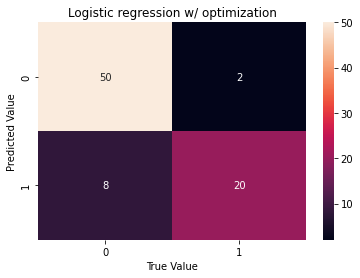
\includegraphics[width=0.5\textwidth]{33}
    \caption{Matrica konfuzije za logističku regresiju sa optimizacijom hiperparametrima}
\end{figure}

\subsection{Stablo odlučivanja}
U navedenom izlazu 3. data je analiza evaluacije klasifikatora 
 optimizovanog hiperparametrima koji ishoduju najbolji slučaj: \verb|ccp_alpha=0.1, max_depth=3|.

 Tačnost koja je ukupna dobijena je 89\%. Preciznost 98\% za vrednost klase 0 i 72\% za vrednost klase 1, senzitivnost 86\% za vrednost klase 0 i 95\% za vrednost klase 1, F1-score 92\% za vrednost klase 0 i 82\% za vrednost klase 1.
\begin{lstlisting}[caption=Stablo odlučivanja sa optimizacijom hiperparametara]
Decision Tree prediction:
Best case:
DecisionTreeClassifier(ccp_alpha=0.1, max_depth=3)


              precision    recall  f1-score   support
           0       0.98      0.86      0.92        58
           1       0.72      0.95      0.82        22

    accuracy                           0.89        80
   macro avg       0.85      0.91      0.87        80
weighted avg       0.91      0.89      0.89        80


\end{lstlisting}

Za izlaz 4. tačnost koja je ukupna dobijena je 88\%. Preciznost 96\% za vrednost klase 0 i 71\% za vrednost klase 1, senzitivnost 86\% za vrednost klase 0 i 91\% za vrednost klase 1, F1-score 91\% za vrednost klase 0 i 80\% za vrednost klase 1.

\begin{lstlisting}[caption=Stablo odlučivanja bez optimizacija hiperparametara]
Decision Tree prediction without optimization:

              precision    recall  f1-score   support
           0       0.96      0.86      0.91        58
           1       0.71      0.91      0.80        22

    accuracy                           0.88        80
   macro avg       0.84      0.89      0.85        80
weighted avg       0.89      0.88      0.88        80
\end{lstlisting}

S obzirom da je izlaz 3. bolji od izlaza 4. daje se prikaz matrice konfuzije za njega na slici 5.

\begin{figure}[h!]
    \centering
    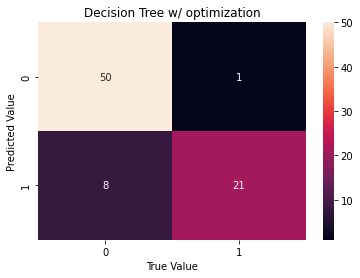
\includegraphics[width=0.5\textwidth]{34.png}
    \caption{Matrica konfuzije za stablo odlučivanja sa optimizacijom hiperparametrima}
\end{figure}

\subsection{Slučajna šuma}

U navedenom izlazu 5. data je analiza evaluacije klasifikatora 
 optimizovanog hiperparametrima koji ishoduju najbolji slučaj: 
 
 \verb|max_depth=10, min_samples_split=10, n_estimators=12|.

 Tačnost koja je ukupna dobijena je 89\%. Preciznost 98\% za vrednost klase 0 i 72\% za vrednost klase 1, senzitivnost 86\% za vrednost klase 0 i 95\% za vrednost klase 1, F1-score 92\% za vrednost klase 0 i 82\% za vrednost klase 1.
\begin{lstlisting}[caption=Slučajne šume sa optimizacijom hiperparametara]
   Random Forest prediction:
Best case:
RandomForestClassifier(max_depth=10, min_samples_split=10, n_estimators=12)

              precision    recall  f1-score   support
           0       0.98      0.86      0.92        58
           1       0.72      0.95      0.82        22

    accuracy                           0.89        80
   macro avg       0.85      0.91      0.87        80
weighted avg       0.91      0.89      0.89        80

\end{lstlisting}

Za izlaz 6. tačnost koja je ukupna dobijena je 89\%. Preciznost 98\% za vrednost klase 0 i 72\% za vrednost klase 1, senzitivnost 86\% za vrednost klase 0 i 95\% za vrednost klase 1, F1-score 92\% za vrednost klase 0 i 82\% za vrednost klase 1.

\begin{lstlisting}[caption=Slučajne šume bez optimizacija hiperparametara]
Random Forest prediction without optimization:
              precision    recall  f1-score   support
           0       0.98      0.86      0.92        58
           1       0.72      0.95      0.82        22

    accuracy                           0.89        80
   macro avg       0.85      0.91      0.87        80
weighted avg       0.91      0.89      0.89        80
\end{lstlisting}

Ista je analiza ishoduje za obe evaluacije da bude ista, pa će u obzir biti uzeta mojim odabirom prvi slučaj na slici 6.

\begin{figure}[h!]
    \centering
    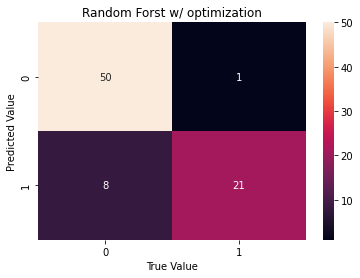
\includegraphics[width=0.5\textwidth]{35}
    \caption{Matrica konfuzije za slučajnu šumu sa optimizacijom hiperparametrima}
\end{figure}

\subsection{Naivni Bajes}
\subsubsection{Gausov Naivni Bajes}
U navedenom izlazu 7. data je analiza evaluacije klasifikatora 
 optimizovanog hiperparametrima koji ishoduju najbolji slučaj koji nije poznat po datom \verb|var_smoothing|-u.
 
 Tačnost koja je ukupna dobijena je 90\%. Preciznost 95\% za vrednost klase 0 i 79\% za vrednost klase 1, senzitivnost 91\% za vrednost klase 0 i 86\% za vrednost klase 1, F1-score 93\% za vrednost klase 0 i 83\% za vrednost klase 1.

\begin{lstlisting}[caption=Gausov naivni Bajes sa optimizacijom hiperparametara]
Gaussian Naive Bayes prediction:
Best case:
GaussianNB()
              precision    recall  f1-score   support
           0       0.95      0.91      0.93        58
           1       0.79      0.86      0.83        22

    accuracy                           0.90        80
   macro avg       0.87      0.89      0.88        80
weighted avg       0.90      0.90      0.90        80
\end{lstlisting}

Za izlaz 8. tačnost koja je ukupna dobijena je 90\%. Preciznost 95\% za vrednost klase 0 i 79\% za vrednost klase 1, senzitivnost 91\% za vrednost klase 0 i 86\% za vrednost klase 1, F1-score 93\% za vrednost klase 0 i 83\% za vrednost klase 1.

\begin{lstlisting}[caption=Gausov naivni Bajes bez optimizacija hiperparametara]
Gaussian Naive Bayes prediction without optimization:

              precision    recall  f1-score   support
           0       0.95      0.91      0.93        58
           1       0.79      0.86      0.83        22

    accuracy                           0.90        80
   macro avg       0.87      0.89      0.88        80
weighted avg       0.90      0.90      0.90        80
\end{lstlisting}


Ista je analiza ishoduje za obe evaluacije da bude ista, pa će u obzir biti uzeta mojim odabirom prvi slučaj slici 7.

\begin{figure}[h!]
    \centering
    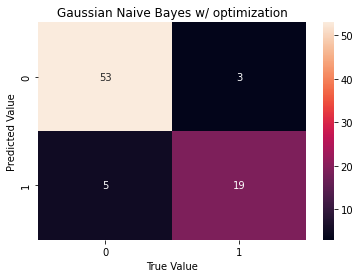
\includegraphics[width=0.5\textwidth]{36}
    \caption{Matrica konfuzije za Gausov naivni Bajes sa optimizacijom hiperparametrima}
\end{figure}

\subsubsection{Multinomijalni naivni Bajes}

U navedenom izlazu 9. data je analiza evaluacije klasifikatora 
 optimizovanog hiperparametrima koji ishoduju najbolji slučaj: \verb|alpha=0.1|
 
 Tačnost koja je ukupna dobijena je 73\%. Preciznost 74\% za vrednost klase 0 i 50\% za vrednost klase 1, senzitivnost 95\% za vrednost klase 0 i 14\% za vrednost klase 1, F1-score 83\% za vrednost klase 0 i 21\% za vrednost klase 1.

\begin{lstlisting}[caption=Multinomijalni naivni Bajes sa optimizacijom hiperparametara]
Multinomial Naive Bayes prediction:
Best case:
MultinomialNB(alpha=0.1)

              precision    recall  f1-score   support
           0       0.74      0.95      0.83        58
           1       0.50      0.14      0.21        22

    accuracy                           0.73        80
   macro avg       0.62      0.54      0.52        80
weighted avg       0.68      0.72      0.66        80
\end{lstlisting}

Za izlaz 10. tačnost koja je ukupna dobijena je 73\%. Preciznost 74\% za vrednost klase 0 i 50\% za vrednost klase 1, senzitivnost 95\% za vrednost klase 0 i 14\% za vrednost klase 1, F1-score 83\% za vrednost klase 0 i 21\% za vrednost klase 1.

\begin{lstlisting}[caption=Multinomijalni naivni Bajes bez optimizacije hiperparametara]
Multinomial Naive Bayes prediction without optimization:

              precision    recall  f1-score   support
           0       0.74      0.95      0.83        58
           1       0.50      0.14      0.21        22

    accuracy                           0.73        80
   macro avg       0.62      0.54      0.52        80
weighted avg       0.68      0.72      0.66        80
\end{lstlisting}

Gausov naivni Bajes se pokazao kao bolji Naivni Bajes klasifikator, pa tako da se samo posmatra matrica konfuzije za njega.

\subsubsection{Bernulijev naivni Bajes}

U navedenom izlazu 11. data je analiza evaluacije klasifikatora 
 optimizovanog hiperparametrima koji ishoduju najbolji slučaj: \verb|alpha=0.1|
 
 Tačnost koja je ukupna dobijena je 73\%. Preciznost 72\% za vrednost klase 0 i 0\% za vrednost klase 1, senzitivnost 100\% za vrednost klase 0 i 0\% za vrednost klase 1, F1-score 84\% za vrednost klase 0 i 0\% za vrednost klase 1.

\begin{lstlisting}[caption=Bernuli naivni Bajes sa optimizacijom hiperparametara]
Bernoulli Naive Bayes prediction:
Best case:
BernoulliNB(alpha=0.1)

              precision    recall  f1-score   support
           0       0.72      1.00      0.84        58
           1       0.00      0.00      0.00        22

    accuracy                           0.73        80
   macro avg       0.36      0.50      0.42        80
weighted avg       0.53      0.72      0.61        80
\end{lstlisting}

Za izlaz 12. tačnost koja je ukupna dobijena je 73\%. Preciznost 72\% za vrednost klase 0 i 0\% za vrednost klase 1, senzitivnost 100\% za vrednost klase 0 i 0\% za vrednost klase 1, F1-score 84\% za vrednost klase 0 i 0\% za vrednost klase 1.

\begin{lstlisting}[caption=Bernuli naivni Bajes bez optimizacija hiperparametara]
Bernoulli Naive Bayes prediction without optimization:


              precision    recall  f1-score   support
           0       0.72      1.00      0.84        58
           1       0.00      0.00      0.00        22

    accuracy                           0.73        80
   macro avg       0.36      0.50      0.42        80
weighted avg       0.53      0.72      0.61        80
\end{lstlisting}

Gausov naivni Bajes se pokazao kao bolji Naivni Bajes klasifikator, pa tako da se samo posmatra matrica konfuzije za njega.

\subsubsection{Kategorički naivni Bajes}

U navedenom izlazu 13. data je analiza evaluacije klasifikatora 
 optimizovanog hiperparametrima koji ishoduju najbolji slučaj: \verb|alpha=0.1|
 
 Tačnost koja je ukupna dobijena je 82\%. Preciznost 92\% za vrednost klase 0 i 64\% za vrednost klase 1, senzitivnost 83\% za vrednost klase 0 i 82\% za vrednost klase 1, F1-score 87\% za vrednost klase 0 i 72\% za vrednost klase 1.

\begin{lstlisting}[caption=Kategorički naivni Bajes sa optimizacijom hiperparametara]
Best case:
CategoricalNB(alpha=0.1)

              precision    recall  f1-score   support
           0       0.92      0.83      0.87        58
           1       0.64      0.82      0.72        22

    accuracy                           0.82        80
   macro avg       0.78      0.82      0.80        80
weighted avg       0.85      0.82      0.83        80
\end{lstlisting}

Tačnost koja je ukupna dobijena je 81\%. Preciznost 88\% za vrednost klase 0 i 65\% za vrednost klase 1, senzitivnost 86\% za vrednost klase 0 i 68\% za vrednost klase 1, F1-score 87\% za vrednost klase 0 i 67\% za vrednost klase 1.
 
\begin{lstlisting}[caption=Kategorički naivni Bajes bez optimizacijom hiperparametara]
Categorical Naive Bayes prediction without optimization:

              precision    recall  f1-score   support
           0       0.88      0.86      0.87        58
           1       0.65      0.68      0.67        22

    accuracy                           0.81        80
   macro avg       0.76      0.77      0.77        80
weighted avg       0.82      0.81      0.81        80
\end{lstlisting}
Gausov naivni Bajes se pokazao kao bolji Naivni Bajes klasifikator, pa tako da se samo posmatra matrica konfuzije za njega.

\subsubsection{Komplementarni naivni Bajes}

U navedenom izlazu 15. data je analiza evaluacije klasifikatora 
 optimizovanog hiperparametrima koji ishoduju najbolji slučaj: \verb|alpha=0.1|
 
 Tačnost koja je ukupna dobijena je 57\%, \textbf{što je najgori ishod nekog klasifikatora zasnovanog na Naivnom Bajesu, a i u celom radu}. Preciznost 68\% za vrednost klase 0 i 46\% za vrednost klase 1, senzitivnost 57\% za vrednost klase 0 i 58\% za vrednost klase 1, F1-score 62\% za vrednost klase 0 i 51\% za vrednost klase 1.

\begin{lstlisting}[caption=Komplementarni naivni Bajes sa optimizacijom hiperparametara]
    Complement Naive Bayes prediction:
    Best case:
    ComplementNB(alpha=0.1)
    
                  precision    recall  f1-score   support
               0       0.68      0.57      0.62        49
               1       0.46      0.58      0.51        31
    
        accuracy                           0.57        80
       macro avg       0.57      0.58      0.57        80
    weighted avg       0.60      0.57      0.58        80
\end{lstlisting}

Za izlaz 16. tačnost koja je ukupna dobijena je 57\%. Preciznost 68\% za vrednost klase 0 i 46\% za vrednost klase 1, senzitivnost 57\% za vrednost klase 0 i 58\% za vrednost klase 1, F1-score 62\% za vrednost klase 0 i 51\% za vrednost klase 1.

\begin{lstlisting}[caption=Komplementarni naivni Bajes bez optimizacije hiperparametara]
Complement Naive Bayes prediction without optimization:
    
                  precision    recall  f1-score   support
    
               0       0.68      0.57      0.62        49
               1       0.46      0.58      0.51        31
    
        accuracy                           0.57        80
       macro avg       0.57      0.58      0.57        80
    weighted avg       0.60      0.57      0.58        80
\end{lstlisting}

Gausov naivni Bajes se pokazao kao bolji Naivni Bajes klasifikator, pa tako da se samo posmatra matrica konfuzije za njega.

\subsection{Mašine potpornih vektora (SVM)}
U navedenom izlazu 19. data je analiza evaluacije klasifikatora 
 optimizovanog hiperparametrima koji ishoduju najbolji slučaj: \verb|C=0.1, gamma=1, kernel='linear'|

Tačnost koja je ukupna dobijena je 85\%. Preciznost 94\% za vrednost klase 0 i 68\% za vrednost klase 1, senzitivnost 84\% za vrednost klase 0 i 86\% za vrednost klase 1, F1-score 89\% za vrednost klase 0 i 76\% za vrednost klase 1.

\begin{lstlisting}[caption=SVM sa optimizacijom hiperparametara]
SVM prediction:
Best case:
SVC(C=0.1, gamma=1, kernel='linear')

              precision    recall  f1-score   support
           0       0.94      0.84      0.89        58
           1       0.68      0.86      0.76        22

    accuracy                           0.85        80
   macro avg       0.81      0.85      0.83        80
weighted avg       0.87      0.85      0.85        80
\end{lstlisting}

Za izlaz 20. tačnost koja je ukupna dobijena je 81\%. Preciznost 82\% za vrednost klase 0 i 77\% za vrednost klase 1, senzitivnost 95\% za vrednost klase 0 i 45\% za vrednost klase 1, F1-score 88\% za vrednost klase 0 i 57\% za vrednost klase 1.


\begin{lstlisting}[caption=SVM bez optimizacije hiperparametara]
SVM prediction without optimization:

              precision    recall  f1-score   support
           0       0.82      0.95      0.88        58
           1       0.77      0.45      0.57        22

    accuracy                           0.81        80
   macro avg       0.80      0.70      0.73        80
weighted avg       0.81      0.81      0.80        80
\end{lstlisting}

S obzirom da je izlaz 19. bolji od izlaza 20. daje se prikaz matrice konfuzije za njega na slici 8.

\begin{figure}[h!]
    \centering
    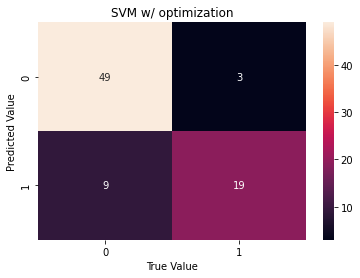
\includegraphics[width=0.5\textwidth]{37.png}
    \caption{Matrica konfuzije za SVM sa optimizacijom hiperparametrima}
\end{figure}

\subsection{K-Najbližih suseda (kNN)}
U navedenom izlazu 21. data je analiza evaluacije klasifikatora 
 optimizovanog hiperparametrima koji ishoduju najbolji slučaj: 
 
 \verb|leaf_size=20, metric='chebyshev', n_neighbors=1, p=1|

Tačnost koja je ukupna dobijena je 86\%. Preciznost 94\% za vrednost klase 0 i 70\% za vrednost klase 1, senzitivnost 86\% za vrednost klase 0 i 86\% za vrednost klase 1, F1-score 90\% za vrednost klase 0 i 78\% za vrednost klase 1.

\begin{lstlisting}[caption=kNN sa optimizacijom hiperparametara]
KNN prediction:
Best case:
KNeighborsClassifier(leaf_size=20, metric='chebyshev', n_neighbors=1, p=1)

              precision    recall  f1-score   support
           0       0.94      0.86      0.90        58
           1       0.70      0.86      0.78        22

    accuracy                           0.86        80
   macro avg       0.82      0.86      0.84        80
weighted avg       0.88      0.86      0.87        80
\end{lstlisting}

Za izlaz 22. tačnost koja je ukupna dobijena je 86\%. Preciznost 93\% za vrednost klase 0 i 72\% za vrednost klase 1, senzitivnost 88\% za vrednost klase 0 i 82\% za vrednost klase 1, F1-score 90\% za vrednost klase 0 i 77\% za vrednost klase 1.

\begin{lstlisting}[caption=kNN bez optimizacije hiperparametara]
KNN prediction without optimization:

              precision    recall  f1-score   support
           0       0.93      0.88      0.90        58
           1       0.72      0.82      0.77        22

    accuracy                           0.86        80
   macro avg       0.82      0.85      0.83        80
weighted avg       0.87      0.86      0.87        80
\end{lstlisting}
S obzirom da je izlaz 21. bolji od izlaza 22. daje se prikaz matrice konfuzije za njega na slici 9.

\begin{figure}[h!]
    \centering
    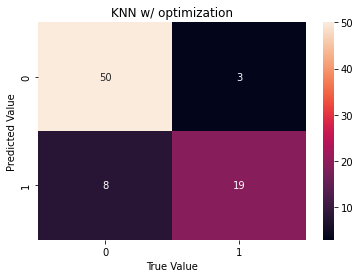
\includegraphics[width=0.5\textwidth]{38.png}
    \caption{Matrica konfuzije za kNN sa optimizacijom hiperparametrima}
\end{figure}

\newpage
\section{Zaključak}
Predstavljeni slučajevi tačnosti za svaki model klasifikacije na tabeli 1. može se uočiti da je najbolji model Gausov naivni Bajes. Sa druge strane, je najgori komplementarni Naivni Bajes. 

Takođe je moguće uočiti da su optimizacije hiperparametrima bile beznačajne kod modela slučajnih šuma, Gausovog, multinomijalnog, Bernulijevog, komplementarnog naivnog Bajesa.



\begin{table}[h]
    \centering
    \begin{tabular}{|r|c|c|}
    \hline
    \textbf{Klasifikator} & \textbf{Tačnost sa GridSearchCV} & \textbf{Tačnost bez GCV} \\
    \hline
    Logistička Regresija & 88\% & 73\% \\
    \hline
    Stablo odlučivanja & 88\% & 73\% \\
    \hline
    Slučajne šume & 89\% & 89\% \\ 
    \hline
    Gaus naivni Bajes & 90\% & 90\% \\ 
    \hline
    Multinomijani naivni Bajes & 73\% & 73\% \\ 
    \hline
    Bernulijev naivni Bajes & 73\% & 73\% \\ 
    \hline
    Kategorički naivni Bajes & 82\% & 81\% \\ 
    \hline
    Komplementarni naivni Bajes & 57\% & 57\% \\ 
    \hline
    SVM & 85\% & 81\% \\ 
    \hline
    KNN & 86\% & 86\% \\ 
    \hline
    \end{tabular}
    \caption{Prikaz tačnosti klasifikatora sa i bez primene optimizacije hiperparametara.} 
\end{table}

%%%%%%%%%%%%%%%%%%%%%%%%%%%%%%%%%%%%%%%%%%%%%%%%%%%%

% \cite{humancpu}

% \subsection{\normalsize{Pogled na pojmove inteligencije, znanja, ljudske imitacije}}
% \subsubsection{\normalsize{Istorija temelja veštačke inteligencije}}



% \begin{enumerate}
    % \item [3.]{\textbf{Da li uticaj misli tradicionalnog zapadnog sveta obazirale su se nad pitanjem odnosa tela i uma kao: 
    % bla bla

    % \item[5.] {\textbf{Moja lična zahtevanja oko inteligencije računarkog softvera.}}
    % bla bla

% \end{enumerate}
\newpage

\begin{thebibliography}{1}
    \bibitem{dataset}
    Social Network Ads, \url{https://www.kaggle.com/datasets/akram24/social-network-ads}, Datum poslednjeg pristupa: \today
    \bibitem{mojRad}
    Ž. Simić, (2024), ``Teorijski izveštaj o klasifikacionim algoritmima sa nadgledanim učenjem'', Univerzitet u Kragujevcu
    \bibitem{pandasDF}
    DataFrame, \url{https://pandas.pydata.org/docs/reference/frame.html}, Datum poslednjeg pristupa: \today
    \bibitem{labelEncoding}
    sklearn.preprocessing.LabelEncoder, \url{https://scikit-learn.org/stable/modules/generated/sklearn.preprocessing.LabelEncoder.html}, Datum poslednjeg pristupa: \today
    \bibitem{train_test_split}
    {sklearn.model\_selection.train\_test\_split}, \url{https://scikit-learn.org/stable/modules/generated/sklearn.model_selection.train_test_split.html}, Datum poslednjeg pristupa: \today
    \bibitem{pairplot}
    seaborn.pairplot, \url{https://seaborn.pydata.org/generated/seaborn.pairplot.html}, Datum poslednjeg pristupa: \today
    \bibitem{displot}
    seaborn.displot, \url{https://seaborn.pydata.org/generated/seaborn.displot.html}, Datum poslednjeg pristupa: \today
    \bibitem{LR}
    sklearn.linear\_model.LogisticRegression, \url{https://scikit-learn.org/stable/modules/generated/sklearn.linear\_model.LogisticRegression.html#sklearn.linear_model.LogisticRegression}, Datum poslednjeg pristupa: \today
    \bibitem{GCV}
    sklearn.model\_selection.GridSearchCV, \url{https://scikit-learn.org/stable/modules/generated/sklearn.model\_selection.GridSearchCV.html}, Datum poslednjeg pristupa: \today
    \bibitem{npLogspace}
    numpy.logspace, \url{https://numpy.org/doc/stable/reference/generated/numpy.logspace.html}, Datum poslednjeg pristupa: \today
    \bibitem{DT}
    sklearn.tree.DecisionTreeClassifier, \url{https://scikit-learn.org/stable/modules/generated/sklearn.tree.DecisionTreeClassifier.html#sklearn.tree.DecisionTreeClassifier}, Datum poslednjeg pristupa: \today
    \bibitem{RFC}
    sklearn.ensemble.RandomForestClassifier, \url{https://scikit-learn.org/stable/modules/generated/sklearn.ensemble.RandomForestClassifier.html}, Datum poslednjeg pristupa: \today
    \bibitem{GNB}
    sklearn.naive\_bayes.GaussianNB, \url{https://scikit-learn.org/stable/modules/generated/sklearn.naive\_bayes.GaussianNB.html#sklearn.naive\_bayes.GaussianNB}, Datum poslednjeg pristupa: \today
    \bibitem{MNB}
    sklearn.naive\_bayes.MultinomialNB, \url{https://scikit-learn.org/stable/modules/generated/sklearn.naive\_bayes.MultinomialNB.html}, Datum poslednjeg pristupa: \today
    \bibitem{BNB}
    sklearn.naive\_bayes.BernoulliNB, \url{https://scikit-learn.org/stable/modules/generated/sklearn.naive\_bayes.BernoulliNB.html}, Datum poslednjeg pristupa: \today
    \bibitem{CNB}
    sklearn.naive\_bayes.ComplementNB, \url{https://scikit-learn.org/stable/modules/generated/sklearn.naive\_bayes.ComplementNB.html}, Datum poslednjeg pristupa: \today
    \bibitem{CatNB}
    sklearn.naive\_bayes.CategoricalNB, \url{https://scikit-learn.org/stable/modules/generated/sklearn.naive\_bayes.CategoricalNB.html}, Datum poslednjeg pristupa: \today
    \bibitem{SVC}
    sklearn.svm.SVC, \url{https://scikit-learn.org/stable/modules/generated/sklearn.svm.SVC.html#sklearn.svm.SVC}, Datum poslednjeg pristupa: \today
    \bibitem{kNN}
    sklearn.neighbors.KNeighborsClassifier, \url{https://scikit-learn.org/stable/modules/generated/sklearn.neighbors.KNeighborsClassifier.html}, Datum poslednjeg pristupa: \today
    \bibitem{metrics1}
    Machine Learning Model Evaluation Metrics part 2: Multi-class classification, \url{https://www.mariakhalusova.com/posts/2019-04-17-ml-model-evaluation-metrics-p2/}, Datum poslednjeg pristupa: \today
    \bibitem{metrics2}
    Classification metrics: Multiclass and multilabel classification, \url{https://scikit-learn.org/stable/modules/model_evaluation.html#multiclass-and-multilabel-classification}, Datum poslednjeg pristupa: \today
\end{thebibliography}

% \title{Seminarski rad}
% \subtitle{Razvoj i oblasti veštačke inteligencije}
% \date{}
% \author{}

% ja ne razumem nista

% {Seminarski rad} \hfill ovo radi \hfill student: Željko Simić

% \hfill what's up?
% \maketitle


% eyo


\end{document}